%% Example of a LaTeX source file for a COLING-2012 submission
%% last updated: July 10, 2012
%% Optional instructions for authors within the tex file are provided as comments and start with 'for authors:...'
\documentclass[10pt,a5paper,twoside]{article}
\usepackage{coling2012}
\usepackage{wrapfig}
\usepackage{amsmath}
\usepackage{latexsym}
\usepackage{xspace}
\usepackage{relsize}
\usepackage{graphicx}
\usepackage{threeparttable}
\usepackage{multirow}
\usepackage[algoruled,vlined]{algorithm2e}
\usepackage{tikz}
\usetikzlibrary{automata}

\newcommand{\tup}[1]{\langle #1 \rangle}
\newcommand{\puse}{\ensuremath{\textsf{p}_\textit{use}}}
\newcommand{\randomuse}{\ensuremath{\textsf{rnd}_\emph{use}}\xspace}
\newcommand{\incuse}{\ensuremath{\textsf{inc}_\emph{use}}\xspace}
\newcommand{\RE}{\textsf{RE}\xspace}
\newcommand{\REL}{\textsf{REL}\xspace}
\newcommand{\IR}{\textrm{I}\!\textrm{R}}
\newcommand{\gM}{\mathcal{M}}
\newcommand{\el}{\ensuremath{\mathcal{EL}}\xspace}
\newcommand{\interp}[1]{|\!|#1|\!|}


\title{Probabilistic Refinement Algorithms\\for the Generation of Referring Expressions}
%for authors: in case of more than four author names ref. to commented line below 
%\author{$Annie~SMITH^{1, 2}~~~LI~Xiao Dong^{1, 3}$\\$~~~Third~Author^{1, 2}~~~Fourth~Author^{1, 3}~~~ Fifth~Author^{2, 3}$\\
\author{$Romina~Altamirano^{1}~~~Carlos~Areces^{1,2}~~~Luciana~Benotti^{1}$\\
{\small  	(1) FaMAF, Universidad Nacional de C\'ordoba, Argentina\\
(2) Consejo Nacional de Investigaciones Científicas y Técnicas, Argentina\\ 
  \texttt{\small \{ialtamir,areces,benotti\}@famaf.unc.edu.ar} \\ 
}}

\begin{document}
\maketitle
%% The first mandatory ABSTRACT (\abstractEn) section below is for the English language
\abstractEn{We propose an algorithm for the generation of referring expressions (REs) that adapts the approach of~\shortcite{arec2:2008:Areces,arec:usin11} 
to include overspecification and probabilities learned from corpora.  After introducing the algorithm, we discuss how probabilities required as 
input can be computed for any given domain for which a suitable corpus of REs is available, and how the probabilities can be adjusted for new scenes in the domain using a machine learning approach.  We exemplify how to compute probabilities over the GRE3D7 corpus of~\shortcite{viet:gene11}.
The resulting algorithm is able to generate different referring expressions for the same target with a frequency similar to that observed in corpora. %Moreover, the most frequently generated referring expressions not in the corpus are also semantically natural, indicating that the algorithm can generalize from the learning data. \\
We empirically evaluate the new algorithm over the GRE3D7 corpus, and show that the probability distribution of the generated referring expressions match the one found in the corpus with high accuracy.}

%for authors: for keywords section either use \keywordsEn OR \keywordsOL below as relevant
%Example for English only keywords list
\keywordsEn{Generation of referring expressions, refinement algorithms, machine-learning}

\newpage



%1. Generation of Referring Expresions
%2. Adding non-determisnism
%p_use es la probabilidad de usar la propiedad si elimina distractores. 
%3. Learning probabilities from corpus
%4. Adding overspecification
%5. Evaluation
%6. Discussion of Non Determinism and Overspecification
%7. Conclusions

\section{Generation of referring expressions}\label{sec:gre}

In linguistics, a \emph{referring expression} (RE) is an expression that 
unequivocally identifies the intended target to the interlocutor, from a set of possible distractors.  
For example, if we intend to identify a certain animal $d$ from a set of pets, the expression 
``the dog'' will be an RE if $d$ is the only dog in the set, and if we are confident
that our interlocutor will identify $d$ as a dog. 

The generation of referring expressions (GRE)  is a key task of most natural 
language generation (NLG) systems (see, e.g.,~\cite[Section 5.4]{dale2000}). 
Depending on the information available to the NLG system, certain objects might 
not be associated with an identifier which can be easily recognized by the user. 
In those cases, the system will have to generate a, possibly complex, description that contains 
enough information so that the interlocutor will be able to identify the intended referent.

The generation of referring expressions is a well developed field in automated natural language generation.
Building upon Dale and Reiter's foundational work~\cite{dale89cooking,Dale1995},
various proposals have investigated the generation of different kinds of referring expressions 
such as relational expressions (``the blue ball next to the cube''~\cite{dale91:_gener_refer_expres_invol_relat}),
reference to sets (``the two small cubes''~\cite{Stone2000}), or more expressive logical connectives (``the 
blue ball not on top of the cube''~\cite{deemter02:_gener_refer_expres}).

REs involving relations, in particular, have
received increasing attention recently; especially in the context of
spatial referring expressions in situated generation (e.g., \cite{kelleher06:_increm_gener_of_spatial_refer}), where it is
particularly natural to use expressions involving spatial relations such as ``the ball on top of the cube.''  However, the classical algorithm by~\shortcite{dale91:_gener_refer_expres_invol_relat} was shown to be unable to generate satisfying REs in practice (see the 
analysis over the \emph{cabinet corpus} in~\cite{viethen06:_algor_for_gener_refer_expres}).  Furthermore, the Dale
and Haddock algorithm and many of its successors (such as~\cite{kelleher06:_increm_gener_of_spatial_refer}) are vulnerable to
the problem of \emph{infinite regress}, where the algorithm enters an infinite loop, jumping back
and forth between descriptions for two related individuals, as in ``the book on the table which supports a book on the
table \ldots''

\shortcite{arec2:2008:Areces,arec:usin11} have proposed new, low complexity algorithms for the generation 
of relational REs (including references to sets) that eliminate the risk of infinite regression. 
These algorithms are based on different variations of the partition refinement algorithms of~\shortcite{paig:thre87}.
The information provided by a given scene is interpreted as a relational model.  The algorithm, then, classifies the 
objects in the model  into sets that can 
be described by the same description.  This classification is successively \emph{refined} (while possible) till the target 
is the only element fitting the description of its class.  The existence of such RE will 
depend, on the one hand, on the information available in the input scene, and on the other 
on the expressive power of the formal language used to describe the elements of the different 
classes in the refinement (e.g., whether the REs can contain negations, or relational information). 

The idea of using a formal language to describe the information that an RE should convey has been discussed 
already in~\cite{Krahmer2003,gardent07:_gener_bridg_defin_descr}.  In~\cite{arec2:2008:Areces,arec:usin11} the 
combination of partition refinement algorithms and different formal languages is used to classify existing 
GRE approaches in an expressiveness hierarchy.  For instance, the classical Dale and Reiter algorithms
compute purely conjunctive formulas; \cite{deemter02:_gener_refer_expres} extends this language by
adding the other propositional connectives, whereas~\cite{dale91:_gener_refer_expres_invol_relat} extends it by
allowing existential quantification.

The refinement algorithms presented in~\cite{arec2:2008:Areces,arec:usin11} effectively
compute REs for all individuals in the domain, at the same time.  The algorithm always terminates, and on termination it returns a formula of 
the formal language chosen that uniquely describes the target, if such a formula exists (i.e., if the 
formal language chosen is expressive enough to uniquely identify the target in the input model). \shortcite{arec2:2008:Areces}
show that the refinement algorithm using the description language \el as formal language is capable of generating 67\% of 
the relational REs in the~\cite{viethen06:_algor_for_gener_refer_expres} dataset, when all possible orders of the relations in the domain are considered. This is in sharp contrast with the analysis 
done in~\cite{viethen06:_algor_for_gener_refer_expres} over the cabinet corpus, of algorithms based in Dale and Reiter's original proposal.    

As mentioned, refinement algorithms require an 
ordered list of the properties that can be used to described the objects in the scene, and the coverage results reported over Viethen and 
Dale's cabinet corpus means that \emph{some ordering} produces a reasonably wide coverage.  In other words, it has been shown that refinement algorithms have the capacity of producing REs similar to those produced by human subjects, provided a suitable ordering over relations appearing 
in the input scene is available, but it is unclear which of all possible orders should be used.  In this article we directly address this issue.  

Our goal is actually twofold. First we show how we can add non-determinism to the refinement algorithms, by replacing the fixed ordering 
over the properties of the input scene by a \emph{probability of use} for each property, and modifying the algorithm accordingly.  
In this way, each call to the algorithm can produce different REs for the same input scene and target.  We will then show that given suitable corpora of REs (like the GRE3D7 corpora discussed in~\cite{viet:gene11}) we can estimate these probability of use so that REs are generated with a probability distribution that matches those found in the corpora.  

The rest of the paper is structured as follows. In Section~\ref{sec:algorithm} we introduce the technical details of the 
refinement algorithms presented in~\cite{arec2:2008:Areces,arec:usin11} and show how to introduce non-determinism using 
the probability of use of the properties in the input scene.  In this section, we assume that these probabilities are provided as 
input to the algorithm. In Section~\ref{sec:learning}, we show how to estimate the 
probability of use of a property from training data. Given corpora consisting of pairs (scene, target) together with the REs used to 
describe the target in each case, we propose a method to compute the probability of use of each property for each scene, and use a machine learning approach to generalize these properties to new targets and scenes not appearing in the corpora. 

Preliminary testing of the resulting algorithms shows that there is still one factor missing to property account for the REs found in corpora: overspecification.  Refinement algorithms only allow a mild form of over-specification in the REs produced.  We discuss this in Section~\ref{sec:overspecification} and propose a modification that let the algorithm generate overspecified, but non trivially redundant RE.  The modification proposed is inspired by the work of~\shortcite{keysar:Curr98}, on the egocentric basis of language.  
Section~\ref{sec:evaluation} presents a quantitative evaluation of the resulting algorithm and discusses interesting examples. We show that when trained with scenes from the GRE3D7 corpora the algorithm can generate REs with a probability distribution that, in certain scenes, coincides with an up to 84.15\% of accuracy with the probability distribution of REs used by humans for that scene. 

In Section~\ref{sec:discussion} we discuss previous work, applications and further motivations for our proposal, focusing on recent work discussing the role of non-determinism and over-specification in the generation of referring expressions. Section~\ref{sec:conclusion} concludes the article and points to future work.


\section{The algorithm}
\label{sec:algorithm}

\fxnote{Romina workign here}

%\newcommand{\REL}{\textsf{REL}\xspace}
%\newcommand{\IR}{\textrm{I}\!\textrm{R}}
%\newcommand{\puse}{\textit{p}\_\textit{use}}
%\newcommand{\pdisc}{\textit{p}\_\textit{disc}}

The algorithm is a modification of the algorithm presented by \cite{arec2:2008:Areces}

We are trying to have an algorithm that generate a reference expresion for a target element in a fixed situation, like in the picture. 
\begin{figure}[htb]
\centering
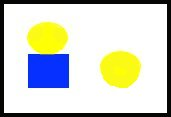
\includegraphics[angle=0,width=0.3\linewidth]{yellowBallBlueCube}
\caption{ 
\label{figura1}
Example figure
}
\end{figure}
The element that we are try to generate a reference expresion has properties and relation with others elements. Let's go to call this description ``the model'', that model can be in xml format like the following example.
\begin{verbatim}
<problem refer-to="b1">
  <individual id="b1">
    <predicate="yellow" />
    <predicate="bowl" />
    <related="above" to="b3"/>
  </individual>
  <individual id="b2">
    <predicate="yellow" />
    <predicate="bowl" />
  </individual>
  <individual id="c">
  </individual>
  <individual id="b3">
    <predicate="blue" />
    <predicate="cube" />
    <related="bellow" to="b1"/>
  </individual>
</problem>
\end{verbatim}
The first thing that we saw is there are algorithms that gives all properties of element before give a relation with another elements, but it see not human. A human can use relations, properties but there is not standard form of use, it mean not everytimes human use properties or relation it depends of the situation. In order to take into account this problem and give more human reference expresion we modify the model for give the same importance to properties and relation, we create a dummy element wich is going to be related to each elements with te relation of the properties that the elements has, it mean every property is going to be a relation with the dummy element ``c'' like we show in the example.

\begin{verbatim}
<problem refer-to="b1">
  <individual id="b1">
    <related rel="yellow" to="c" />
    <related rel="bowl" to="c" />
  </individual>

  <individual id="b2">
    <related rel="red" to="c" />
    <related rel="bowl" to="c" />
  </individual>

  <individual id="b3">
    <related rel="blue" to="c" />
    <related rel="cube" to="c" />
    <related="bellow" to="b1" />
  </individual>
  
  <individual id="c">
  </individual>
</problem>
\end{verbatim}

and plus, we use the probabilities for properties and relation calculated from a human corpora.
With this background we explain the algorithm.

$\REL$ is the set of relation symbols in the signature. It include the properties that are right now relation to the dummy simbol ``c''. 

For each $R \in \REL$ we asume defined two values $R.\puse \in \IR$, the 
probability of using relation $R$ in a RE; and $R.\pdisc \in \IR$, the 
probability that the hearer recognizes relation $R$. 

The algorithm compute the $\mathcal{L}$-similarity sets from a model. 
We are going to have 2 set of formulas, the first one set of formulas are that have not overspecification, and give the limit of iterations of the program, and the second one set of formulas gives overspecification for some elements in case that they run enough for found them.

We calculate two random numbers for each relation, those random numbers are fixed for the entire execution, one for use an another for discernibility. 

it mean that we want not to re-calculate the random in each time for relation, it is like a human don't chance your main of if a word is used or not and if it is discernible or not.

How the algorithm take the goal?
While there is change in the first set os formulas, for each of the relation ordered by higher probability of use, if the probability of use if higher than random probability of the relation for each partition at the moment if the probability of discernibility is higher than the random probability of the relation we add the informatives formulas of each side of set of formulas, but if the discernibility probability of the relation is less than the random probability for that relation we only add the formula to the right side, it is the side that have overspecification.
When no chance of the left side is made the algorithm finish. You can see that sometimes the algorithm generate one overspecification and finish because not see change in the left side, it is to prevent the non-termination of the algorithm.


\begin{algorithm}[h]
\dontprintsemicolon
\caption{Computing the $\mathcal{L}$-similarity sets}\label{algo:bisim-l}
\KwIn{A model $\gM = (\Delta, \interp{\cdot})$ , a list $Rs \in (\REL \times I\!\!R)^*$
 of relation symbols with their \puse values
}
\KwOut{A set of formulas \RE such that
$\{\interp{\varphi} \mid \varphi \in \RE\}$ is the set of
$\mathcal{L}$-similarity 
sets of $\gM$.}

$\RE \leftarrow \{\top\}$

\For{$(R,R.\puse) \in Rs$}{
	$R.\randomuse$ = Random()\\
}
\While{$\exists \varphi \in \RE. |\interp{\varphi_O}|>1$}{
    \RE' $\leftarrow$ \RE \;
    \For{$(R, R.\puse) \in Rs$}{
        \If{$R.\randomuse \le R.\puse$}{
            \For{$\varphi \in \RE$}{
                add$_\mathcal{L}(R, \varphi, \RE)$}
                }\;
            \If{\RE $\not =$ \RE'}{exit}
            }
   \If{\RE $=$ \RE'}{exit}
}
\end{algorithm}

\begin{algorithm}[h]
\dontprintsemicolon
\caption{add$_\el(R, \varphi, \RE)$} \label{algo:bisim-add-el}
\If{$R.\randomdisc \le R.\pdisc$}{
\For{$(\psi_O,\psi_R) \in \RE$ with $|\interp{\psi_O}| > 1$}{
  \If{$\psi_O \sqcap \exists R.\varphi_O$ is not subsumed in $\RE$ {\bf and}
    $\interp{\psi_O \sqcap \exists R.\varphi_O} \neq \emptyset$ {\bf and}
    $\interp{\psi_O \sqcap \exists R.\varphi_O} \neq \interp{\psi_O}$}{
    add $(\psi_O \sqcap \exists R.\varphi_O, \psi_R \sqcap \exists R.\varphi_R)$ to $\RE$ \;
    remove subsumed formulas from $\RE$\;
  }
}
}
\Else{
%\For{$(\psi_O,\psi_R) \in \RE$ with $|\interp{\psi_O}| > 1$}{
%  \If{
%    $\interp{\psi_R \sqcap \exists R.\varphi_R} \neq \emptyset$}
%    {
%    add $(\psi_O, \psi_R \sqcap \exists R.\varphi_R)$ to $\RE$ \;
%    }
\For{$(\psi_O,\psi_R) \in \RE$ with $|\interp{\psi_O}| > 1$}{
  \If{%$\psi_O \sqcap \exists R.\varphi_O$ is not subsumed in $\RE$ {\bf and}
    $\interp{\psi_R \sqcap \exists R.\varphi_R} \neq \emptyset$ {\bf and}
    $\interp{\psi_R \sqcap \exists R.\varphi_R} \neq \interp{\psi_R}$}{
    add $(\psi_O, \psi_R \sqcap \exists R.\varphi_R)$ to $\RE$ \;
    %remove subsumed formulas from $\RE$\; No borramos porque no afectamos a fiO
    }
  }
}
\end{algorithm}


\section{Learning to describe new objects from corpora}
\label{sec:learning}

In the previous section we presented an algorithm that assumes that each relation R 
used in a referring expressions has a known probability of use R.\puse. In this section, 
we describe how to calculate these probabilities from corpora.  
The general set up is the following: we assume available a corpus of REs associated 
to different scenes that are typical of the domain in which the GRE algorithm will have to operate.   
We show first how to calculate R.\puse\ values for those scenes for which a corpus of REs is available.  
We then show how to generalize these values to 
other scenes in the domain, using a machine learning algorithm. \textit{First we} will exemplify the methodology using 
the GRE3D7 corpus which we introduce in the Section ~\ref{sec:learningGRE} and then we will show how to do the same with the TUNA-corpus 
that we describe in Section~\ref{sec:learningTUNA}.

\subsection{\textit{The GRE3D7:} A corpus of referring expressions}
\label{sec:learningGRE}

The GRE3D7 corpus of~\shortcite{viet:gene11} consists of 4480 referring expressions. 
It is the largest corpus of distinguishing descriptions developed to date. 
The REs in the corpus describe objects in 32 3D scenes. Each scene contains a small number of simple objects 
(cubes and balls), and the individual descriptions were elicited in the absence of a preceding discourse. 
The stimulus scenes are designed in a way that encourage the use of relations between objects, but do not require them 
(i.e., a purely propositional RE for the target always exists). For a detailed description of the collection procedure 
see~\cite[Chapter 5]{viet:gene11}. A sample scene used in the corpus collection is shown in Figure~\ref{GRE3D7-stimulus} 
(the target object is marked with an arrow). Table~\ref{corpus-distribution} shows the REs that appear in the corpus for 
Figure~\ref{GRE3D7-stimulus} together with their total number of occurrences and the percentage these totals represent.  

\begin{table}[h!]
\begin{center}
\begin{tabular}{|l|c|c|}
\hline
Referring expressions & Occurrences & Percentage \\
\hline
green ball & 91 & 65.00\% \\
small green ball & 23 & 16.43\% \\
small green ball on top of large blue cube & 8 & 5.71\% \\
green ball on top of blue cube & 5 & 3.57\% \\
green ball on top of large blue cube & 5 & 3.57\% \\
small green ball on top of blue cube & 2 & 1.43\% \\
ball on top of cube & 1 & 0.71\% \\
small green ball on top of large blue cube to the left & 1 & 0.71\% \\
small ball on top large cube & 1 & 0.71\% \\
green ball on top & 1 & 0.71\% \\
small ball on top of small cube & 1 & 0.71\% \\
green ball on top of cube & 1 & 0.71\% \\
\hline
\end{tabular}
\caption{Referring expressions produced by the subjects for Figure~\ref{GRE3D7-stimulus}\label{corpus-distribution}}
\end{center}
\end{table}

The REs in the corpus were produced by 294 participants, each participant producing 16 referring expressions corresponding to 16 
different scenes. In this way, 140 descriptions for each of the 32 scenes were obtained, resulting in a corpus of 4480 REs in total. 

\fxnote{Add closing paragraph}

\subsection{\textit{The TUNA-corpus: A corpus of referring expressions}}
\label{sec:learningTUNA}

\textit{The ASGRE Challenge used the TUNA Corpus (Gatt
et al., 2007), a set of human-produced referring expressions (REs) for entities in visual domains of
pictures of furniture or people. The corpus was
collected during an online elicitation experiment in
which subjects typed descriptions of a target referent
in a DOMAIN in which there were also 6 other entities (‘distractors’). 
Each scene is an XML file that contains the target and distractors with theirs properties, the RE given for a human, and the annotation of this.   
For the challenge 780 singular descriptions in the corpus were used, and divided
into 60\% training data, 20\% development data and
20\% test data. Participants were given both input
(DOMAIN) and output (DESCRIPTION) parts in the
training and development data, but just inputs in the
test data.}


\subsection{Calculating \puse\ when a corpus for the scene is available}

Suppose we want to automatically generate REs for target $t$ in a given scene, and that we do have available a corpus $C$ 
of REs for $t$ in that scene (this is exactly the kind of information we find in the GRE3D7 corpus \textit{and in the TUNA-corpus}).  
We use the REs in $C$ to define the relational model 
used by the algorithm.  Then we estimate the value of \puse\ for each of the relations in the model as the percentage of REs 
in which the relation appears.  I.e., 
\begin{equation}\label{eq1}
R.\puse = \frac{\# \mbox{ of REs in $C$ in which R appears}}{\# \mbox{ of REs in $C$}}.
\end{equation}

\noindent
This estimation is overly simplified and, for example, it does not differentiate between the properties of a target and the 
properties of a landmark object used in a relational RE to complete the description of the target.  But it is extremely easy 
to compute, and we will see in Section~\ref{sec:evaluation} that it already produces natural REs that match those found in the corpus. 

To clarify the computation of R.\puse\ and the model $\gM$ associated to each scene we list the required steps in detail, 
and discuss how we carried them out in the GRE3D7 corpus:

\vspace*{-.4cm}
\begin{enumerate}
\item Tokenize the referring expressions and call the set of tokens $T$. In particular, multi-word expressions like ``on top of'' 
should be matched to a single token like \emph{ontop}.\\[-1.9em]

\item Remove hyperonyms from $T$. E.g., if both \emph{cube} and \emph{thing} appear in $T$, delete \emph{thing}.\\[-2em]

\item If the set of tokens obtained in the previous steps contains synonyms normalize them to a representative in the synonym class, 
and call the resulting set $\REL$; it will be the signature of the model $\gM$ used by the algorithm. E.g., the tokens \emph{little} 
and \emph{small} are both represented by the token \emph{small}.\\[-1.9em]

\item For each scene, define $\gM$ such that the interpretation $\interp{\cdot}$ ensures that all the REs in the corpus are REs in the model.
 E.g., the $\el$ formulas corresponding to the REs in Table~\ref{corpus-distribution} should all denote the target in the model $\gM$ 
depicted in 
Figure~\ref{GRE3D7-stimulus-graph}.\\[-1.9em]

\item For each R $\in \REL$ compute R.\puse\ using~(\ref{eq1}).\\[-1.9em]

\end{enumerate}

Steps 1-5 above are easy to carry out (actually, the tokenization and normalization steps were already done in the GRE3D7 corpus). 
Starting from the scene in Figure~\ref{GRE3D7-stimulus} and the corresponding corpus shown in Table~\ref{corpus-distribution}, 
the resulting signature and their associated \puse\ are listed in the first three columns of Table~\ref{probability-of-use}. 

Notice that the values R.\puse\ obtained in this way should be interpreted as the probability of using R to describe the target in model 
$\gM$, and we could argue that they are correlated to the \emph{saliency} of R in the model.  
For that reason, for example, the value of \emph{ball}.\puse\ is 1, while the value of \emph{cube}.\puse\ is 0.178.  
These probabilities will not be useful to describe different targets in different scenes.  We will see how we can use them to obtain
 values for new targets and scenes using a machine learning approach in the next section.  Not surprisingly, using these values for 
R.\puse\ the REs generated most often by the algorithm can be found in the corpus.  More interestingly, as we discuss in 
Section~\ref{sec:evaluation} the algorithm generates REs with a distribution that matches the one found in the corpus and, 
as Table~\ref{results-algo-fig3} shows, even the generated REs not found in the corpus are natural.    


\subsection{Calculating \puse\ for scenes without corpora for the target} \label{subsec:learning}

If there is no corpora that describes the target we can estimate the \puse from corpora on a different scenes in the same domain. 

We use simple features to obtain the function, all the features can be extracted automatically from the relational model 
and are listed 
in Table~\ref{features}.  

\begin{small}
\begin{table}[h!]
\begin{center}
\begin{tabular}{|l|p{10cm}|}
\hline
target & whether the target element has the property \\
\#rel-prop & number of properties and relations that the target has\\
\#rel & number of the relations that the target has \\
landmark & whether a landmark of the target has the property, an object is a landmark if there is a direct relation in the model 
between them \\
discrimination & 1 over the number of objects in the model that have the property \\
\hline
\end{tabular}
\caption{Features used for learning the \puse ~for each token in the signature of the scenes \textit{(GRE3D7 and TUNA-corpus)} \label{features}}
\end{center}
\end{table}
\end{small}

Our feature set is intentionally simplistic in order for it to be domain independent. As a result there are some complex relations 
between characteristics of the scenes that it is not able to capture. The most important characteristic of the GRE3D7 domain is that we are not able 
to learn, and has an impact in our performance, the properties of type size (namely, small and large) are used much more 
when the target cannot be uniquely identified with taxonomical (ball and cube) and absolute (green and blue) properties only. 
In other words, in the GRE3D7 corpus the size is used more often (90.2\%) of the time when the resulting RE is not overspecified 
than when it is (34\%). It may not be possible to learn this characteristic from the GRE3D7 data since even with the domain dependent 
features defined in~\cite[Chapter 6]{viet:gene11}, it could not be learned by decision trees. As a result we can see in 
Table~\ref{probability-of-use} that for Fig 13 the value estimated for ``large'' are not close to the value calculated from corpora. 
\textit{In the case of the TUNA-corpus we show that we couldn't learn the dependency of dimension-x and dimension-y, it mean, when a person adds 
dimension-x is highly probably that he includes dimension-y in his referring expression.}
\begin{table}[h!]
\begin{center}
\begin{tabular}{|l|c|c|c|c|}
\hline
Token & Model Fig 3 \puse & Learned Fig 3\puse & Model Fig 13 \puse & Learned Fig 13 \puse \\
\hline
ball & 1.0 & 1.0 & 1.0 & 1.0 \\
cube & 1.0 & 1.0 & 1.0 & 1.0 \\
green & 0.978 & 0.993 & 1.0 & 0.9875 \\
small & 0.257 & 0.346 & 0.0428 & 0.1993 \\
on-top & 0.178 & 0.179 & 0 & 0\\ 
blue & 0.15 & 0.124 & 0.064 & 0.1353 \\
large & 0.107 & 0.03 & 0.307 & 0.7378 \\
left & 0.007 & 0.002 & 0 & 0.0024 \\
top & 0.007 & 0 & 0 & 0 \\
right & 0 & 0.001 & 0.064 & 0.0005 \\
left-of & 0 & 0 & 0 & 0 \\
right-of & 0 & 0 & 0.064 & 0.1023 \\
below-of & 0 & 0 & 0 & 0 \\
\hline
\end{tabular}
\caption{Probabilities of use of the tokens from the corpora in Table~\ref{GRE3D7-stimulus}  \textit{(GRE3D7)} \label{probability-of-use}}
\end{center}
\end{table}

The learning was done with the machine learning toolkit WEKA~\cite{Hall:WEK09}, training on all minus one 
(the one for that we are learning) for all the scenes of the GRE3D7 \textit{and the TUNA-corpus}. 
We use linear regression to learn the function of \puse\ for each word in the signature.
For a given scene, we replace the variables of the obtained function by the values of the features in the scene 
that we want to describe.

\textit{Using} linear regression we are able to learn interesting characteristics of the domain. To start with, it learns known facts such that the 
saliency of a color depends strongly on whether the target object is of that color, and it does not depend on its discrimination power 
in the model. Moreover, it learns that the on-top relation is used more frequently than the horizontal relations (left-of and right-of) 
which confirms a previous finding reported in~\cite{viet:gene11}. Finally, it learned a surprising fact of the GRE3D7 corpus
 (not found by previous work), that is that size is used more frequently in an overspecified manner when the target and landmark share the
 size. Size was used in overspecified REs in 49\% of the descriptions for scenes where target and landmark shared the size, and 25\% 
of the time when target and landmark did not share the size. This can be explained by the observation that if landmark and target share a
 property, this property is more salient. 


%\section{Generating overspecified descriptions} \label{sec:overspecification}

As it stand, Algorithm~\ref{algo:bisim-l} allows very little overspecification in the REs it
generates.  A relation with a low \puse\ might be enough by 
(by itself or in combination with some of the relations already considered) to 
identify the target. Once this relation is added, we obtain an RE, but a shorter, 
more specific RE might be possible, by eliminating some of the previous refinements. 
Hence, the resulting RE might be overspecified. This is the same kind of overspecification 
that the original incremental algorithm allows.  But it has been argued~\cite{Engelhardt_Bailey_Ferreira_2006,Arts_Maes_Noordman_Jansen_2011} that 
a might higher degree of overspecification is usually found in corpora, and this 
is indeed what can be seen in the GRE3D7 corpus.  As we can see in Table~\ref{corpus-distribution}, 
the target is described 16.43\% of the times as a ``small green ball'' when ``green 
ball'' is already an RE.  Using the \puse\ values learnt from the calculus explained
in the previous section, Algorithm~\ref{algo:bisim-l} cannot simulate this behavior. 

Because the fundamental idea of the algorithm is semantics, handling overspecification in 
a natural way is difficult. If two properties have the same interpretation in a given 
model, then once the first has been considered the second will not refine the classes 
obtained so far, and hence the algorithm won't include it in the generated descriptions. 
On the other hand, if we disregard the condition the informativeness constrain (i.e., 
the fact that the addition of a relation indeed refine the class, eliminating some of 
the elements it contains), then we run the risk of generating descriptions like ``the green 
green ball.''

As a compromise, we consider the following variation of Algorithm~\ref{algo:bisim-l} were 
we disregard the informativeness constrain (i.e., we allow the inclusion of new relations 
in the description, even if they do not refine the associated class) \emph{but only during the 
first loop of the algorithm}.  That is, during the first loop over the elements in the 
input list Rs, we will allow the inclusion of all relations that do not trivialize the 
description (i.e., the associated class is not empty).  Because this is done only during 
the first loop, we know that repeated properties will not appear in the generated REs.  
In the remaining loops, additional properties will be added only if they are informative. 
The modified algorithm is shown in Figure~\ref{fig:algo3}.

\begin{figure}[t]
\small
\centering
\begin{algorithm}[H]
\dontprintsemicolon
\caption{add$_\el$(R, $\varphi$, \RE)} \label{algo:bisim-add-el-over}

\eIf(\tcp*[f]{\footnotesize are we in the first loop?}){\em FirstLoop?}{
    Informative $\leftarrow$ $\top$ \tcp*[f]{\footnotesize allow overspecification}}{
    Informative $\leftarrow$ $\interp{\psi \sqcap \exists \mbox{\em R}.\varphi} \neq \interp{\psi}$ \tcp*[f]{\footnotesize informative: smaller than the original?}}
\For{\em $\psi \in$ \RE with $|\interp{\psi}| > 1$}{
  \If{\em $\psi \sqcap \exists$R.$\varphi$ is not subsumed in \RE\ {\bf and} \tcp*[f]{\footnotesize non-redundant: can't be obtained form \RE?}\\
    \em \ \ \ $\interp{\psi \sqcap \exists \mbox{\em R}.\varphi} \neq \emptyset$ {\bf and} \tcp*[f]{\footnotesize non-trivial: has elements?}\\
     \ \ \  \emph{Informative}}{
    add $\psi \sqcap \exists \mbox{R}.\varphi$ to $\RE$ \tcp*[f]{\footnotesize add the new class to the classification} \;
    remove subsumed formulas from $\RE$ \tcp*[f]{\footnotesize remove redundant classes}
  }
}
\end{algorithm}
\vspace*{-.5cm}\caption{Refinement function with overspecification for the \el-language}\label{fig:algo3}
\end{figure}

Clearly, Algorithm~\ref{algo:bisim-add-el-over} does not capture all possible forms of overspecification, but as we will see in the next section it does account for most of the kinds of overspecification found in the GRE3D7 corpus.  

\section{Evaluation} \label{sec:automaticeval}

We perform two kinds of evaluation a first one to compare the output of our system with the best results of the ASGRE challenge 2008, using automatic metrics provided in the challenge for comparison and the second one is a human evaluation we ask to two judges to select the best RE we will show that the judges prefered the system generated RE.

In order to perform the evaluation we take the development part of the TUNA corpus as test, it includes 80 RE for pictures of Furniture  and 60 RE for pictures of People.

\subsection{Automatic evaluation}

ACA ME GUSTARIA EXPLICAR MEJOR LAS METRICAS, Y EXPLICAR ALGO BASICO DE GRAPH

Using \puse~learned as described in Section~\ref{sec:learning} and running our algorithm 100 times, then we order from high to low the ouput of the system, so we have a list of RE with his respectives frequencies we call the most frequent RE SYS\_furniture\_1 for Furniture scenes and SYS\_People\_1 for People scenes, including the second more frequent we call SYS\_furniture\_2 and SYS\_people\_2 and so on until 20 including the 20th RE we call SYS\_furniture\_20 and SYS\_people\_20 then we use execute the automatic evaluation with the automatic metrics of the ASGRE challenge. 
In the challenge they calculate minimality, defined as the proportion of descriptions produced by a system
that are maximally brief, as per the original definition in Dale (1989). The Dice coefficient, used to compare the description produced by a system to the human-produced description on the same input domain. %Dice is estimated
MASI, a version of the Jaccard similarity coefficient proposed
by Passonneau (2006) which multiplies the similarity value by a monotonicity coefficient, biasing
the measure towards those cases where DS and
DH have an empty set difference. Intuitively, this
means that those system-produced descriptions are
preferred which do not include attributes that are
omitted by a human. Thus, two of our intrinsic measures assess Humanlikeness (Dice and MASI), while
Minimality reflects the extent to which an algorithm
conforms to brevity, one of the principles that has
emerged from the ASGRE literature.
Our results are comparable with the best results of the ASGRE challenge (The GRAPH system~\cite{KrahmerGRAPH}), but we also will show in the Section~\ref{sec:evaluation} that the RE generated by te system are more prefered than the humans ones.

In Table~\ref{Tabla_sis_1_20} we show the automatic metrics descripted bellow and comparison with our system the first more frequent and the one that includes the 20 more frequent RE.

\begin{table}[h!]
\begin{center}
\begin{tabular}{|l|c|c|c|c|}
\hline
%Figure & Model \puse &  Learning \puse & Random \puse &  Uniform \puse \\
	 	& 	DICE		&	MASI	&	A\_ACCURACY	&MINIMALITY	\\
\hline
GRAPH Furniture	& 	.80 		&	.59	&	.48		&	.0 	\\
GRAPH People 	& 	.72		&	.48	&	.28		&	.0	\\
\hline
SYS\_Furniture\_1	&	.79		&	.58	&	.43		&	.01	\\
SYS\_People\_1	&	.65		&	.37	&	.19		&	.0	\\
\hline
SYS\_Furniture\_20&	.87		&	.75  	&	.65		&	.01	\\
SYS\_People\_20	&	.81		&	.68	&	.60		&	.01	\\
\hline
\end{tabular}
\vspace*{.1cm}
\caption{Comparison GRAPH and our system the more frequent and the first 20}
\label{Tabla_sis_1_20}
\end{center}
\end{table}
\vspace*{-.9cm}
%Estos son los numeros que obtuve de accuracy para furniture (con estos hice el grafico)
%	GRAPH	OUR SYSTEM
%1	0.48	0.43
%5	0.48	0.5
%10	0.48	0.5375
%15	0.48	0.6
%20	0.48	0.65

% y estos para people
%	GRAPH	OUR SYSTEM
%1	0.28	0.19
%5	0.28	0.42
%10	0.28	0.47
%15	0.28	0.54
%20	0.28	0.6

In the picture~\ref{graficoPresicionFurniture} we can see that taking the first RE our system is a little lower than GRAPH but taking into account the forst 5 more frequent RE given by the system our accuracy is the same of GRAPH, and taking 20 into account our system is as far better, for people in the picture~\ref{graficoPresicionPeople} we can see that even less that 3 we have the same accuracy as GRAPH, and also if we take into account more RE the system is better.

\begin{figure}[ht]
%\begin{minipage}{0.50\linewidth}
\centering
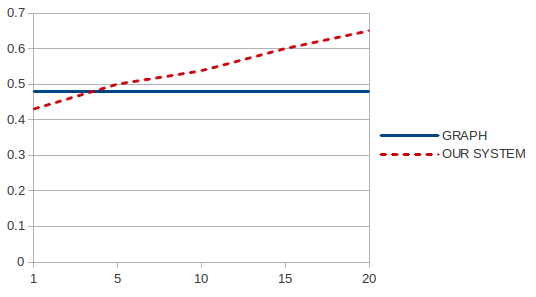
\includegraphics[width=0.8\textwidth]{images/furniturePrec.png}
\caption{Comparison of accuracy of GRAPH and our system for furniture}
\label{graficoPresicionFurniture}
\end{figure}

\begin{figure}[ht]
%\begin{minipage}{0.50\linewidth}
\centering
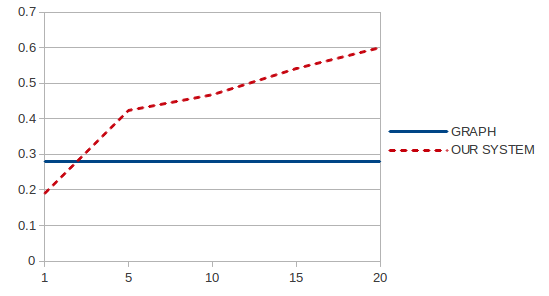
\includegraphics[width=0.8\textwidth]{images/peoplePrec.png}
\caption{Comparison of accuracy of GRAPH and our system for people}
\label{graficoPresicionPeople}
\end{figure}

Also we analyze the the RE founded in the corpus that the system does not generate in a first frequency, and found that there were a 13.75\% in furniture that were not RE, it is were underspecified sentences with does not identifies the target object. For people the proportion was lower just a 5.88\%. We saw that when a person used another word that was not taking in account in the annotation part of the corpus, it was annotated as ``other'', and our system was not capable of generate ``other'' because it was not in the model.
In the table there is a percentage of times that in 100 runs the system does not generates the RE given by the human, as showed in Table~\ref{error-people} the human were more difficult to generate in the first 100 because the RE were longer and when the RE have less probability of occur. If the it system does not generates the RE in 100 of runs does not mean that the system could not generate them, it just mean that the system need to be running more in order to generate this RE.\\


\begin{table}[h!]
\begin{center}
\begin{tabular}{|l|c|c|}
\hline
		& Count		& Percentage\\
\hline
It is not RE	&	11	&	13.75 \\
%		&	37	&	46.25\% \\
Contains ``other''	&	6	&	7.50 \\
\hline
SYS does not generated the RE in 100 runs	&	8	&	10.00 \\
SYS generated but not with higher frequency	&	18	&	22.5 \\
\hline
\end{tabular}
\vspace*{.1cm}
\caption{Clasification of RE that the system could not generates or generates with low frequency for Furniture}
\label{error-people}
\end{center}
\end{table}
\vspace*{-.4cm}

\begin{table}[h!]
\begin{center}
\begin{tabular}{|l|c|c|}
\hline
			& Count		& Percentage\\
\hline
It is not RE		&	4	&	5.88 \\
Contains ``other''	&	6	&	8.82 \\
\hline
SYS does not generated the RE in 100 runs	&	17	&	25.00 \\
SYS generated but not with higher frequency	&	28	&	41.18 \\
%BIEN			&	13	&	19.12\% \\

\hline
\end{tabular}
\vspace*{.1cm}
\caption{Clasification of RE that the system could not generates or generates whit low frequency for People}
\label{error-furniture}
\end{center}
\end{table}
\vspace*{-.4cm}
\subsection{Human evaluation} \label{sec:evaluation}

We aisle the RE that our system gives another RE with more frequency it is that not coincides with the one given by the human in the corpus, and with those realize a human evaluation in order to see if the RE produced by the system are prefered by human than the RE produced by humans. Two judges fluent or natural speakers of English were asked to select the best of each pair of RE.

We have 43 scenes of furniture (from 80) and 55 scene of people (from 68), for which of them we manually realize the referring expressions (including the properties given as results by our algorithm) and ask people to evaluate which one is a RE it is that univocally identifies the target object and wich one is better in sense that will be more usefull for a human who is not seeing the red box to identify the object. For do it we prepare a webpage with each of the pictures and 2 choices randomly ordered human and system RE. Out goal is to try to show if RE produced by our system are at less as good as the produced by human, and also we will show that they are even better.

%\begin{table}[h!]
%\begin{center}
%\begin{tabular}{|c|c|c|c|}
%\hline
%           & Agree in & Not agree & Total\\
%\hline 
%Furniture & 25       & 18        & 43 \\
%People    & 25       & 30        & 55 \\
%Total     & 50       & 48        & 98 \\
%\hline
%\end{tabular}
%\caption{Agree between judges} 
%\label{agree-judges}
%\end{center}
%\end{table}

%esta tabla no ayuda...no se que decir, no se como justificar que no coincidan...
%In the Table~\ref{agree-judges} we can see that the both judges choice the same RE 25 times for Furniture and 25 times for People, 

\begin{table}[h!]
\begin{center}
\begin{tabular}{|c|c|c|c|c|}
\hline
Judge    & Human choice & System choice  & Human choice & System choice \\
	 &    Furniture &    Furniture   &    People    &    People \\
\hline 
Judge1   & .23       & .77      & .45  & .55  \\
Judge2   & .26       & .73      & .41  & .59  \\
\hline
\end{tabular}
\vspace*{.1cm}
\caption{Porcentage of system versus human selected choices for each judge} 
\label{system-versus-human}
\end{center}
\end{table}
\vspace*{-.9cm}
In the Table~\ref{system-versus-human} you can see the judges selected more the RE generated by our system than the human RE.

%\begin{table}[h!]
%\begin{center}
%\begin{tabular}{|c|c|c|c|}
%\hline
%Judge    & Human choice & System choice & Total\\
%\hline 
%Judge1 & 25       & 30        & 55 \\
%Judge2    & 23       & 32        & 55 \\
%\hline
%\end{tabular}
%\caption{System versus human selected choice for People} 
%\label{system-versus-human-people}
%\end{center}
%\end{table}

%In the case of pictures of people you can see in the Table~\ref{system-versus-human-people} that the judges selected more RE generated by our system but the diference in not very significant.

\begin{table}[h!]
\begin{center}
\begin{tabular}{|c|c|c|c|c|c|}
\hline
           & System & System (\%) & Human & Human (\%) & Total\\
\hline
Furniture & 23  & .92 &  2 & .08  & 25 \\
People    & 16  & .64 & 9  & .36 & 25 \\
\hline
Total     & 39  & .78    & 11 & .22 & 50  \\
\hline
\end{tabular}
\vspace*{.1cm}
\caption{Coincidences between judges, the system is the prefered the 78\% of times} 
\label{system-better}
\end{center}
\end{table}
\vspace*{-.9cm}
Taking account just the coincidences between jugdes in average as you can see in the Table~\ref{system-better} they prefered the system in 78\% of times.

Sometimes comparison was unfair because human gives a RE that includes relation that were not annotated so, the system haven't the posibility of produce them. A point in favor of the system is that sometimes the human did an underespecified RE and the system has a better one.\\


Sometimes judges choices the same RE for example in Figure~\ref{smallBlueFan1} the RE given by the human was underspecified, so they choice the system one because was a RE. Another times just RE given by the system was intuitivelly less complex than the human one like in Figure~\ref{smallBlueFan} where RE of the system was ``small blue fan'' and the human RE was ``bottom row, blue fan''.
\begin{figure}[ht]
\begin{minipage}{0.50\linewidth}
\centering
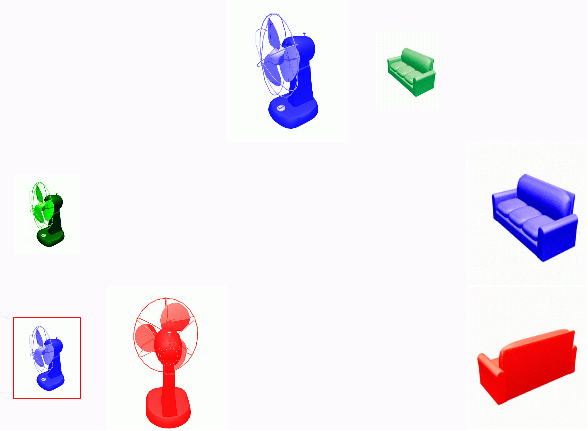
\includegraphics[width=\textwidth]{images/smallBlueFan1.jpg}
\caption{TUNA corpus people scene}
\label{smallBlueFan1}
\end{minipage}
\begin{minipage}{0.50\linewidth}
\centering
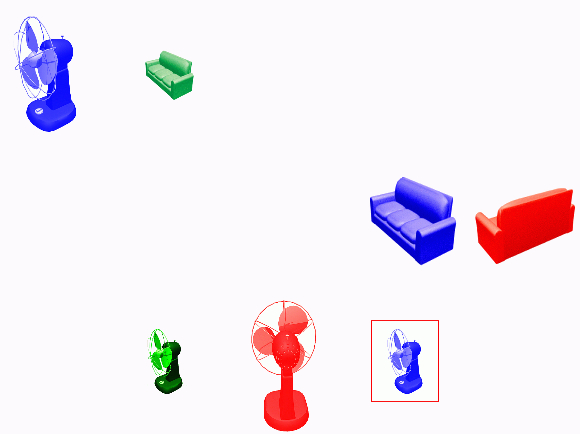
\includegraphics[width=\textwidth]{images/smallBlueFan.jpg}
\caption{TUNA corpus furniture scene}
\label{smallBlueFan}
\end{minipage}
\end{figure}

Sometimes the judges choice the human RE for example in Figure~\ref{largeGreyChair} the
system RE was ``large grey chair facing away'' and the human RE was ``the top left grey chair''.

\begin{figure}[ht]
%\begin{minipage}{0.50\linewidth}
\centering
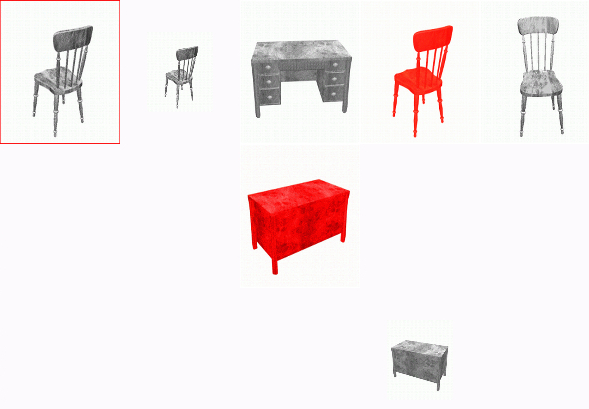
\includegraphics[width=0.8\textwidth]{images/largeGreyChair.jpg}
\caption{TUNA corpus people scene}
\label{largeGreyChair}
\end{figure}


EN HUMAN EVALUATION AGREGAR CASOS EN LOS QUE LOS JUECES CONSISTENTEMENTE ELIGIERON LA EXPRESION DE LA PERSONA Y CASOS EN LOS QUE LOS JUEVES ELIGIERON CONSISTENTEMENTE EXPRESIONES HUMANAS. DAR UNA IDEA DE PORQUE LAS EXPRESIONES DEL SISTEMA SON A VECES MEJORES Y PORQUE A VECES LAS DE LOS HUMANOS SON MEJORES (E.G. DEPENDENCIA ENTRE X E Y)

\section{Discussion and Conclusions} \label{sec:discussion}

We extend~\shortcite{arec2:2008:Areces} algorithm to generate REs similar to those produced by humans. The modifications 
we proposed are based on two observations. First, it has been argued that no fixed ordering of properties is able to generate all REs produced by humans and, second, humans frequently overspecify their REs~\cite{Engelhardt_Bailey_Ferreira_2006,Arts_Maes_Noordman_Jansen_2011,viet:gene11}. We tested 
the proposed algorithm on the GRE3D7 corpus and found that it is able to generate a large proportion of the overspecified REs found in the corpus without generating trivially redundant referring expressions.
%
\shortcite{viet:gene11} trains decision trees that achieve 65\% average accuracy on the GRE3D7 corpus. 
This approach is able to generate overspecified relational descriptions, but they might fail to be referring 
expressions. Indeed, because the  method does not verify the extension of the generated expression over a model of the scene, the 
generated descriptions might not uniquely identify the target.  As we have already discussed,
our algorithm ensures termination and it always finds a referring expression if one exists.  Moreover, it achieves an average of 75\% of accuracy over the 8 scenes used in our tests. 

Different algorithms for the generation of overspecified referring expressions have been recently proposed~\cite{delucena-paraboni:2008:ENLG,ruud-emiel-mariet:2012:INLG2012}.  To our knowledge, they have not been evaluated on the 
GRE3D7 corpus and, hence, comparison is difficult. \shortcite{delucena-paraboni:2008:ENLG} and \shortcite{ruud-emiel-mariet:2012:INLG2012} algorithm
have been evaluated on the TUNA-AR corpus~\cite{gatt-balz-kow:2008:ENLG} where they have achieved a 33\% and 40\% accuracy respectively. 
As the TUNA-AR corpus includes only propositional REs, it would be interesting future work to evaluate how these algorithms perform in corpora with relational REs such as GRE3D7. 


The way we introduce overspecification is inspired by the work of~\shortcite{keysar:Curr98} on egocentrism and natural language production.  Keysar~et al.\ argue that when producing language, considering hearers point of view is not done from the outset but it is rather an afterthought; adult speakers produce REs egocentrically, just like children do, but then adjust REs so that the addressee is able to identify the target unequivocally. The first, egocentric, step is a heuristic process based in a model of saliency of the scene that contains the target. 
Our definition of \puse\ is intended to capture the saliences of the properties for different scenes and targets. The \puse\ of a relation changes according to the scene. This is in contrast with previous work where the saliency of a property is constant in a domain. Keysar et al.~argue that the reason for this generate-and-adjust procedure may have to do with information processing limitations of the mind: if the heuristic that guides the egocentric phase is well tunned, it succeeds with a suitable RE in most cases and seldom requires adjustments. Interestingly, we observe a similar behavior with our algorithm: when \puse\ values learned from the domain are used, the algorithm is not only more accurate but also much faster. 

Besides testing our algorithm over the rest of the scenes in the GRE3D7 corpus, 
as future work we plan to evaluate our algorithm on more complex domains 
like those provided by Open Domain Folksonomies~\cite{pacheco-duboue-dominguez:2012:NAACL-HLT}. We will also 
explore corpora obtained through interaction
such as the GIVE Corpus~\cite{GarGarKolStr10} where it is common to observe multi shot REs. Under time pressure, subjects will first produce an underspecified expression that includes salient properties of the target (e.g., ``the red button'').  And then, in a following utterance, they add additional properties (e.g., ``to the left of the lamp'') to make the expression a proper RE  identifying the target uniquely. The source code and the documentation for the algorithm are distributed under the GNU Lesser GPL and can be obtained at \url{http://code.google.com/p/bisimulation-gre}.

%\section{Conclusions}\label{sec:conclusions}

%\fxnote{\tiny  I would like to rewrite the conclusions also. It reads to weak
%and too vague. Empezar repitiendo cual es el punto principal del paper y cual
%fue la contribucion.  Lo que hay que decir ya esta dicho en lo que esta escrito,
%pero falta decirlo more 'to the point' y sin dar tantas vueltas.}

The content determination phase during the generation of referring
expressions identifies which `properties' will be used to refer to a
given target object or set of objects. What is considered as a
`property' is specified in different ways by each of the many
algorithms for content determination existing  in the literature. In
this article, we put forward that this issue can be addressed by
deciding when two elements should be considered to be equal, that
is, by deciding which discriminatory power we want to use. Formally,
the discriminatory power we want to use in a particular case can be
specified syntactically by choosing a particular formal language, or
semantically, by choosing a suitable notion of simulation.  It is
irrelevant whether we choose first the language (and obtain the
associated notion of simulation afterwards) or vice versa.

We maintain that having both at hand is extremely useful. Obviously,
the formal language will come handy as representation language for
the output to the content determination problem.  But perhaps more
importantly, once we have fixed the expressivity we want to use, we
can  rely on model theoretical results defining the adequate notion
of sameness underlying each language, which indicates what can and
cannot be said (as we discussed in \sect{technical}). Moreover, we
can transfer general results from the well-developed fields of
computational logics and graph theory as we discuss
in~\sect{simulation} and~\sect{krahmer}, where we generalized known
algorithms into \emph{families} of GRE algorithms for different
logical languages. %These notions were crucial also in
%\sect{combining} to devise new heuristics.


%Each language has its own expressive power, and
%this induces an adequate notion of sameness. Naturally this last
%notion becomes crucial when trying to uniquely refer to an element
%in a model.


%We have discussed making the notion of expressiveness involved an
%explicit parameter of the GRE problem, unlike usual practice. Hence
%we talk of ``$\+L$-GRE problem'', for a logical language $\+L$. We
%considered various possible choices for $\+L$, though we did not
%argue for any of them. Instead, we tried to make explicit the
%trade-off involved in the selection of a particular $\+L$. This, we
%believe, depends heavily on the given context.


An explicit notion of expressiveness also provides a
cleaner interface, either between the content determination and
surface realization modules or between two collaborating content
determination modules. An instance of the latter was exhibited in
\sect{combining}.

As a future line of research, one may want to avoid sticking to a
fixed $\+L$ but instead favor an incremental approach in which
features of a more expressive language $\+L_1$ are used only when
$\+L_0$ is not enough to distinguish certain element.

%\fixme{Podemos generalizar el algoritmo para conjuntos? Mencionar algoritmo de Piazza}

%To finish this section, observe that the algorithms introduced here
%can also be used to compute referring expressions for \emph{sets} of
%elements. Let $\+L$ be \EL or \ELAN. For any $v\in\Delta$ we define
%the $\+L$-class of $v$ as
%%\fixme{$[v]_{\+L}$ pide demasiado. alcanza con que sean todos los $u$ tq $v \simul{\+L} u$, no?}
%$$
%[v]_{\+L}=\{u\in\Delta\mid u\in\simset_{\+L}(v)\wedge
%v\in\simset_{\+L}(u)\}.
%$$
%A set $T\subseteq\Delta$ has an $\+L$-RE iff $T=[u]_{\+L}$ for some
%$u\in\Delta$. In case $T=[u]_{\+L}$ for some $u$ then for any
%$v\in[u]_{\+L}$, $F(v)$ is a $\+L$-RE for $T$.
%
%Since computing the $\+L$-classes of $\Delta$ is polynomial in
%$\size{\Delta}$, Theorem \ref{thm:complexity-EL-GRE} implies the
%following:


%\fixme{ARREGLAR} To finish this section, observe that the algorithms
%introduced here can also be used to compute referring expressions
%for some \emph{sets} of elements. Let $\+L$ be \EL or \ELAN. A set
%$T\subseteq\Delta$ has an $\+L$-RE iff $T=\simset_{\+L}(u)$ for some
%$u\in\Delta$. In case $T=\simset_{\+L}(u)$ for some $u$ then $F(u)$
%is a $\+L$-RE for $T$. In fact, $F(v)$ also is, for any $v$ such
%that $u\in\simset_{\+L}(v)\wedge v\in\simset_{\+L}(u)$.

%Hence by Theorem \ref{thm:complexity-EL-GRE} we have:

%\begin{cor}
%The problem of generating the \EL and \ELAN referring expressions of
%sets of elements given a finite model
%%$\gM=\tup{\Delta,\interp{\cdot}}$
%can be solved in polynomial time.
%\end{cor}


\bibliographystyle{apa}

\bibliography{coling2012}

\end{document}\begin{flushleft}\end{flushleft}
